\begin{figure}[t]
\centering
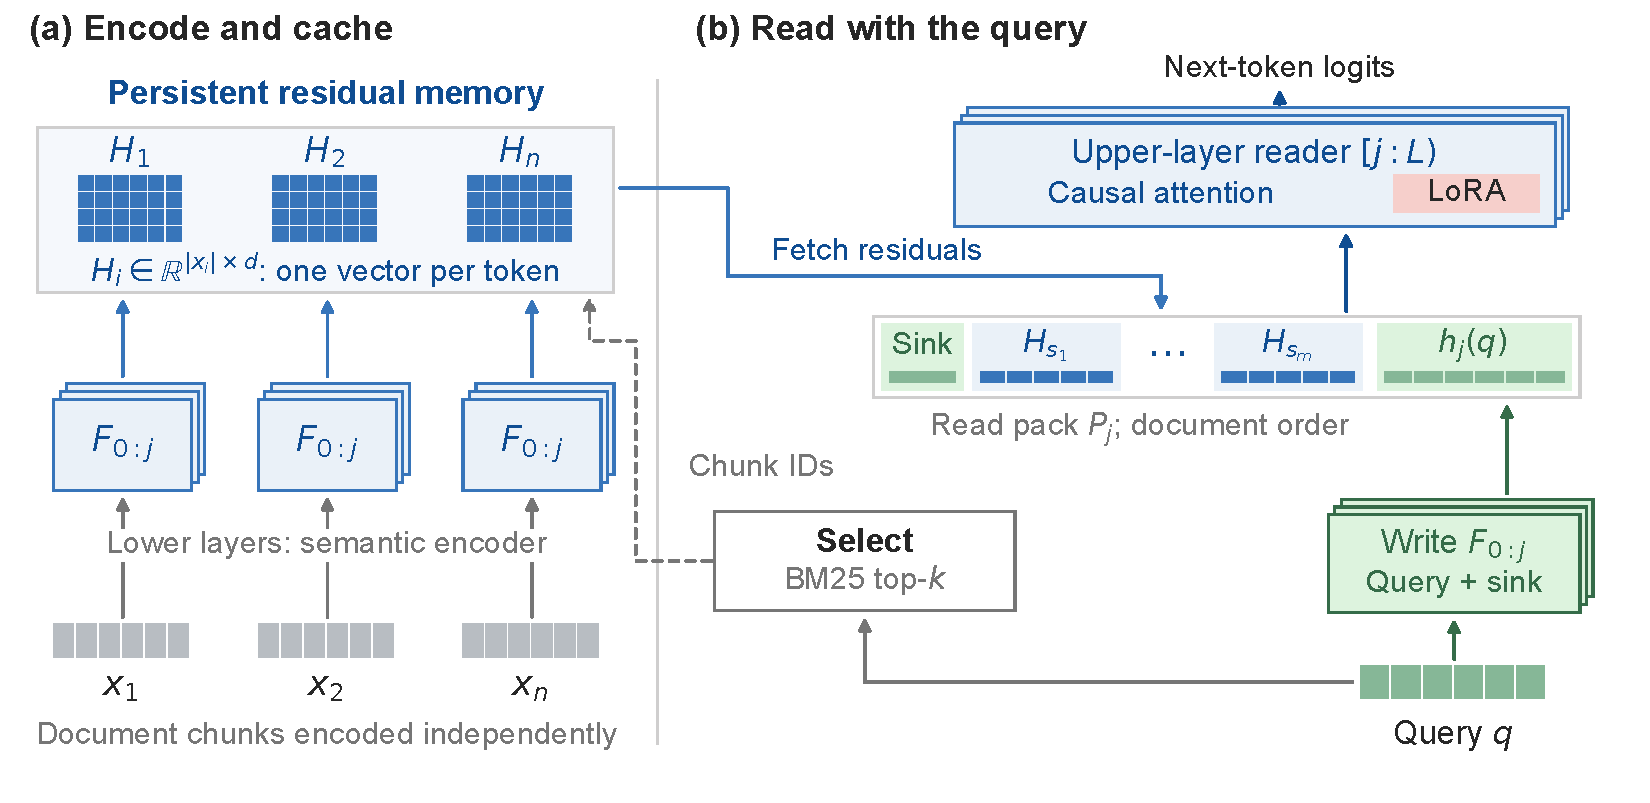
\includegraphics[width=\linewidth]{figures/architecture.pdf}
\caption{\textbf{CoMem reuses document computation at a residual interface.} (a) The shared lower-layer semantic encoder writes each chunk into a residual matrix $H_i$. (b) The query selects at most $k$ chunk IDs (dashed path). Cached encodings (blue) join separately encoded sink/query states (green), in document order, for causal processing by the upper reader $[j{:}L)$. Suffix LoRA adapts this reader to independently written states; the frozen variant omits it. Overlap-Write adds left context in (a) while retaining only target-token states.}
\label{fig:arch}
\end{figure}
